% This is a template by André Greiner-Petter for a PhD thesis.
% The comments starting with "%TODO" mark the blocks you should update
% for your own thesis.

\RequirePackage[utf8]{inputenc}
\RequirePackage[T1]{fontenc}
\documentclass[twoside,titlepage,11pt,a4paper]{book}

%TODO Use the following command \printtrue to activate print colors (e.g., no colored links)
\newif\ifprint
\printfalse
%\printtrue

\usepackage[dvipsnames,table]{xcolor}	% colors
\usepackage{styles/customfields}

%TODO The following fields contains the basic information of your thesis and
% will appear on the front page: 
\title{PhD Thesis Title} % the title of your thesis
\subtitle{Thesis Subtitle} % the subtitle of your thesis
\author{Andr\'{e} Greiner-Petter} % the author
\degree{Doctor of Engineering Sciences (Dr.-Ing.)} % the degree you are going to obtain
\department{School of Electrical, Information and Media Engineering} % the department of your university
\group{Data \& Knowledge Engineering Group} % your research group (this is optional and you can just skip this if you don't have a group)
\logo{logo/BUW_logo.svg.png} % the path to the logo with the university name
\city{Wuppertal} % The city of your university
\submissionyear{2021} % The year of submission

% The following entries are just for the meta data of the generated PDF.
% This ensures a more professional PDF output even though most people will not
% notice it in the end.
\subject{Doctoral Thesis in Scientific Computing, University of Wuppertal, October 2021}
\keywords{First Keyword, 2nd Keyword, Drittes Keyword}

%%%%%%%%%%%%% STANDARD PACKAGES %%%%%%%%%%%%%%%%

% fonts and symbols
\usepackage{lmodern} % backup plan (will be mostly overwritten by libertine)
\usepackage[mono=false]{libertine}

\usepackage{amsthm}
\usepackage{amssymb}
\usepackage{xfrac} % multi additional fracs, such as sfrac
\usepackage{enumitem} % customizable enumerates/itemizes

% since we use libertine, this hack is not needed anymore
%\DeclareFontShape{T1}{lmr}{bx}{sc} { <-> ssub * cmr/bx/sc }{}

% ensure latin modern for tt fonts (verb, codes, etc)
\renewcommand{\ttdefault}{lmtt}

% that should allo urls to break lines
% url gets loaded by other packages later, hyperref, biblatex, etc
% so we use this to force adding the hyphens option to the package
\PassOptionsToPackage{hyphens}{url}

% ------------- COLOR DEFINITIONS ------------- %
\usepackage[dvipsnames,table]{xcolor}	% more colors
\definecolor{RoyalRed}{RGB}{157,16,45}

\definecolor{PrimaryBlue}{HTML}{3C6382}
\definecolor{SecondaryYellow}{HTML}{F6B93B}

\definecolor{DefinitionRed}{HTML}{b71540} % before: b71540
\definecolor{SignalGreenColor}{HTML}{afdd5c}
\definecolor{ParadiseGreenColor}{HTML}{78e08f} % 60a3bc

\colorlet{AccentPrime}{RoyalRed!80!black}
\colorlet{AccentNum}{black}
\colorlet{AccentLine}{PrimaryBlue}
\colorlet{AccentSec}{SecondaryYellow}
\colorlet{LinkPrime}{black}

\colorlet{HighlightCorrectColor}{ParadiseGreenColor!60!white}

\colorlet{CodeBoxColor}{PrimaryBlue}
\colorlet{TranslationBoxColor}{SecondaryYellow}
\colorlet{DefinitionBoxColor}{DefinitionRed}
\colorlet{HighlightScope}{SecondaryYellow!30}

\definecolor{TranslationBoxLightColor}{HTML}{f8ca6d} 
\definecolor{ExampleBoxColor}{HTML}{82ccdd}
\definecolor{ThesisObjectiveBoxColor}{HTML}{78e08f}
\definecolor{ResearchTaskBoxColor}{HTML}{38ada9}

\definecolor{PaperBoxColor}{HTML}{ad5a81} %{B53471} 

\colorlet{TableRowColor}{gray!10!white}
\colorlet{BoxBackgroundColor}{gray!10!white}

\colorlet{exMathColor}{gray!100!white}
\colorlet{exMathColorHighlight}{OrangeRed!80!white}

\colorlet{CorrectBackgroundColor}{OliveGreen!20!white}
\colorlet{CorrectBackgroundDLMFColor}{SpringGreen!90}
\colorlet{WrongBackgroundColor}{Red!20!white}
\colorlet{WrongBackgroundDLMFColor}{Red!20!white}

% standard link colors
\colorlet{citationcolor}{green}
\colorlet{urlcolor}{magenta}

\colorlet{checkMarkColor}{ForestGreen!80!LimeGreen}
\colorlet{crossMarkColor}{Red!80!BrickRed}
\colorlet{crossColor}{Orange}
\colorlet{questionMarkColor}{Red!65}

% printing minimal color settings:
% LinkPrime = black (doc internal links)
% AccentPrime = black (chapter headers)
% AccentLine = black (page number vertical line color on every page)
% below in hypersetup, set citecolor and urlcolor to black
\makeatletter%
\ifprint%
	\colorlet{LinkPrime}{black}
	\colorlet{AccentPrime}{black}
	\colorlet{AccentLine}{gray}
	\colorlet{citationcolor}{black}
	\colorlet{urlcolor}{black}
	
	\colorlet{BoxBackgroundColor}{gray!12!white}
	\colorlet{TableRowColor}{gray!12!white}
	
	%\colorlet{checkMarkColor}{gray}
	%\colorlet{crossMarkColor}{black}
	%\colorlet{crossColor}{black}
	%\colorlet{questionMarkColor}{black}
	
	%\colorlet{CorrectBackgroundColor}{gray!20!white}
	%\colorlet{CorrectBackgroundDLMFColor}{gray!90}
	%\colorlet{WrongBackgroundColor}{gray!20!white}
	%\colorlet{WrongBackgroundDLMFColor}{gray!20!white}
\fi
\makeatother%

% ------------- BIBLIOGRAPHY ------------- %
\usepackage[
	backend		= biber,
	style		= numeric,
	natbib		= true,
	url			= true,
	doi			= true,
	eprint		= false,
	giveninits	= true,
	defernumbers= true, % recommended due to splitting bib in the end
	maxbibnames	= 6,
	minbibnames	= 3,
	sorting		= nty,
	alldates	= iso,
	seconds		= true, % is required when we set date format to 'iso'
	sortcites,
	backref % adds back references to citations in bibliography (very nice)
]{biblatex}

% Bold author positions via author+an = {<numberOfAuthor>=highlight}
\renewcommand*{\mkbibnamegiven}[1]{%
  \ifitemannotation{highlight}%
    {\textbf{#1}}%
    {#1}}

\renewcommand*{\mkbibnamefamily}[1]{%
  \ifitemannotation{highlight}%
    {\textbf{#1}}%
    {#1}}

% control the number of maxbibnames later
\makeatletter
\newcommand\Setmaxbibnames[1]{\renewcommand\blx@maxbibnames{#1}}
\makeatletter

\addbibresource{./bibliography/Bibliography.bib}
\addbibresource{./bibliography/BibliographyISO.bib}

% stop biblatex from redefining markboth
%\defbibheading{subbibintoc}[\refname]{%
%  \addsec{#1}%
%   \markboth{#1}{#1}}% DELETED
%  }% NEW

% allow further stretches for references to avoid overfull hboxes
\emergencystretch=1.5em

% allow line breaks in URLs in bibliography
\apptocmd{\UrlBreaks}{\do\f\do\m}{}{}
\setcounter{biburllcpenalty}{9000}% Kleinbuchstaben
\setcounter{biburlucpenalty}{9000}% Großbuchstaben

% ------------- LANG SPECS ------------- %
% lang settings
\usepackage[%
	main=english, % for some german text
	ngerman, % for \autoref again
	english % obviously the main language we go for
]{babel}

% should be after babel
% see here for the settings: http://www.khirevich.com/latex/microtype/
\usepackage[
	activate={true,nocompatibility},
	tracking=true,
	kerning=true,
	spacing=true,
	factor=1100,
	stretch=15,
	shrink=15
]{microtype}
\microtypecontext{spacing=nonfrench}
\SetTracking{encoding={*}, shape=sc}{40}

\RequirePackage[ 
	autostyle,
	german=quotes,
]{csquotes} % setup proper citations depending on current language

% ------------- LINKS AND TOCS ------------- %
% setup hyperlinks and TOC
\usepackage[pdfpagelabels,plainpages=false]{hyperref}
\usepackage[nohints]{minitoc}
\usepackage[titles]{tocloft}
\usepackage{parskip} % space between paragraphs (after tocloft)

% allow more stretching for URLs to avoid underfull/overfull problems
\Urlmuskip=0mu  plus 5mu

\setcounter{minitocdepth}{3}

% link setup
\makeatletter
\hypersetup{
	%draft		= true,% deleted all links and colors of links! Printing mode
	pdftitle	= {\@title\space --- \@subtitle},
	pdfsubject  = {\@subject},
	pdfauthor	= {\@author},
	pdfcreator	= {\@author},
	pdfkeywords	= {\@keywords},
    colorlinks, % instead of color borders, color the string
    linkcolor	= {LinkPrime}, %{red!0!black} <- print
    citecolor	= {citationcolor}, %{blue!0!black} <- print
    urlcolor	= {urlcolor}
}
\ifprint%
	\hypersetup{
		linkbordercolor=black,
		pdfborderstyle={/S/U/W 1}
	}%
\fi
\makeatother

% ------------- GLOSSARY, FIGURES, STYLES ------------- %
\usepackage[symbols]{glossaries} % generate glossaries (for example acronyms)
% -------------------- DEFINE GLOSSARY ENTRIES ----------------------- %
% In this file you define the glossary entries. There are 2 custom fields
% available. In this template, we do not distinguish between acronyms and
% abbreviations. In turn, if you specify a new glossary entry which is an
% acronym, you must manually add the "first" field to specify how the first
% use of the entry should look like. Typically this is the long version version
% of the acronym followed by the acronym itself, e.g., "Personal Computer (PC)".
% If you want to add the long version of an acronym, use 
% the appropriate custom field user1. If you want to add the definition of
% a math symbol in the glossary, use the custom field user2. 
%
% Important notice, you are not supposed to use user1 and user2 for the same
% entry!
%
% The custom fields are:
%
% 	user1: The long version of an acronym. For example: 
%		name=BLEU,
%		user1={Bilingual Evaluation Understudy}
%
%	user2: Used for the definition of math symbols. For example
%		name={\ensuremath{f(x)}},
%		user2={$x^2$}
%
% Here is a complete example:
%
%\newglossaryentry{id}
%{
%    name=NAME,
%    user1={Non Affirmative Meme Entry},
%    description={The description of the entry},
%    plural={NAMEs}, % the plural form of the entry
%    first={Non Affirmative Meme Entry (NAME)} % if this is an acronym, you may want to define the first usage. The first time you use the entry, it prints the "first" field, all later uses take the "name" field.
%}
% 


\makeglossaries

% -------------------- MATH SYMBOLS ----------------------- %
\newglossaryentry{mbm25-math}
{
    name={\ensuremath{\operatorname{mBM25}(t,d)}},
    user2={$\displaystyle\protect\underset{d \in D}{\operatorname{max}} \frac{\left( k + 1 \right) \operatorname{IDF}(t) \operatorname{ITF}(t,d) \operatorname{TF}(t,d)}{\protect\underset{t' \in d|_{c(t)}}{\operatorname{max}}\! \operatorname{TF}(t',d) + k \left( 1-b + \frac{b \operatorname{AVG}_{\mathrm{DL}}}{|d| \operatorname{AVG}_{C}} \right)}$},
    description={Our mathematical \gls{bm25} ranking to measure the importance of a given \gls{moi} $t$ in a document $d \in D$ which is part of a corpora $D$. $\operatorname{IDF}(t)$ is the inverse-document frequency, $\operatorname{ITF}(t,d)$ the inverse-term frequency of $t$ in $d$, $\operatorname{TF}(t,d)$ the term frequency of $t$ in $d$, $\operatorname{AVG}_{\mathrm{DL}}$ the average document length (number of terms) in $D$, $\operatorname{AVG}_{C}$ the average complexity of terms in $D$, $c(t)$ the complexity of $t$, and $b$, $k$ are parameters}
}

% -------------------- DEFINE ACRONYMS ----------------------- %

\newglossaryentry{moi}
{
    name=MOI,
    user1={Mathematical Objects of Interest},
    description={Is a term referring to subexpressions in mathematical formulae with a specific meaning~\cite{GreinerPetterSMB20}. One can consider these parts as elements of general interest},
    plural={MOIs},
    first={Mathematical Objects of Interest (MOI)}
}

\newglossaryentry{bm25}
{
    name=BM25,
    user1={Okapi BM25},
    description={Is a ranking function to calculate the relevance of results in a search engine~\cite{RobertsonZ09}. The underlying idea of BM25 is that words that appear regularly only in a few documents are more \textit{important} for that document than words that appear everywhere across the entire corpora}
}

\newglossaryentry{www}
{
    name={WWW},
    user1={The Web Conference},
    description={An annual major conference with the focus on the world wide web (has a \gls{core} rank of \texttt{A*})}
}

\newglossaryentry{core}
{
    name={CORE},
    user1={Computing Research and Education Association of Australasia},
    description={Is an association of university departments that provide assessments of major conferences in the computing disciplines. The main categories are \texttt{A*} (flagship), \texttt{A} (excellent), \texttt{B} good to very good, and \texttt{C} for other ranked conferences that meet minimum standards, see \url{http://portal.core.edu.au/conf-ranks/} [accessed 2021-10-01]}
}

\newglossaryentry{scientometrics}
{
    name={Scientometrics},
    description={An international journal with an 5-year \gls{if} of $3.702$ for quantitative aspects of the science of science, communication in science and science policy. According to \url{https://academic-accelerator.com/5-Year-Impact-Factor/Scientometrics} [accessed 2021-10-01] it is placed 18 of 227 journals in the field of library and information sciences}
}

\newglossaryentry{if}
{
    name={IF},
    user1={Impact Factor},
    description={The impact factor of a journal is the number of citations during the past (usually 2 or 5) years divided by the number of published publications in the same time period}
}

% In case you want to add all entries you defined regardless if they appear in your text,
% uncomment the following line:
%\glsaddall

% setup graphics
\usepackage{graphicx}           % for all images
\usepackage{subcaption}             % for subfloats (titlepage images)
\usepackage{wrapfig}			 % wrapping text around figures
\graphicspath{ {./images/} }    % set the default path for graphics

%%%%%%%%%%%%% VISUALS %%%%%%%%%%%%%%%%

\usepackage{tikz}
\usetikzlibrary{arrows.meta}
\usetikzlibrary{calc}
\usetikzlibrary{positioning}

\usepackage{styles/thesis}
\usepackage{styles/modernbox}
\myIconConfiguration{icon/shape = hexagon}

\usepackage{pifont}
\newcommand{\checkMark}{\textcolor{checkMarkColor}{\ding{52}}}
\newcommand{\crossMark}{\textcolor{crossMarkColor}{\ding{56}}}
\newcommand{\cross}{\textcolor{crossColor}{\textbf{\ding{56}}}}
\newcommand{\questionMark}{\textcolor{questionMarkColor}{\textbf{\textsc{?}}}}

\newcommand{\quoteMark}{\textcolor{gray!20}{\scalebox{5.0}{\ding{125}}}}

% alternatives
\newcommand{\correct}{\checkMark}
\newcommand{\maybe}{\questionMark}
\newcommand{\wrong}{\crossMark}

\makeatletter
% #1 is a multiplier of fontsize for the minimum diameter of the circle
% #2 is the symbol to be circled.
\NewDocumentCommand{\circled}{ O{1.6} O{crossMarkColor} m }{%
\tikz[baseline={(char.base)}]{
    \node[shape=circle, draw, inner sep=1pt, 
        minimum height={\f@size*#1}, color=#2] (char) {#3};}}
        
\NewDocumentCommand{\badge}{ m }{%
\tikz[baseline={(char.base)}]{
    \node[shape=circle, draw, inner sep=1pt, line width=.3mm,
        minimum height={\f@size*1.2}, color=CodeBoxColor!80!black, fill=Gray!7] (char) {\textbf{#1}};}}
\makeatother

%%%%%%%%%%%%% CUSTOM MACROS %%%%%%%%%%%%%%%%
\newcommand{\accessed}{[accessed 2021-10-01]}

% command for linking to github issues
\newcommand{\isnr}[1]{\href{https://github.com/ag-gipp/GoUldI/issues/#1}{#1}}
\newcommand{\PPPcite}[1]{\href{#1}{\textcolor{red}{[?]}}}
\newcommand{\qId}[1]{\href{https://mathmlben.wmflabs.org/#1}{#1}}
\newcommand{\qvar}[1]{\ensuremath{\textcolor{red}{#1}}}
\newcommand{\wData}[2][]{\href{https://www.wikidata.org/w/index.php?title=Q#2&oldid=#1}{\texttt{Q#2}}}
\newcommand{\w}[2]{\href{https://www.wikidata.org/wiki/#1}{#2}}

\newcommand{\NN}{{\mathbb N}}
\newcommand{\ZZ}{{\mathbb Z}}
\newcommand{\RR}{{\mathbb R}}
\newcommand{\CC}{{\mathbb C}}

% inline graphics
\newlength\myheight
\newlength\mydepth
\settototalheight\myheight{Xygp}
\settodepth\mydepth{Xygp}
\setlength\fboxsep{0pt}
\newcommand*\inlinegraphics[1]{%
  \settototalheight\myheight{Xygp}%
  \settodepth\mydepth{Xygp}%
  \raisebox{-\mydepth}{\includegraphics[height=\myheight]{#1}}%
}

% use \dlmf{14.4.14} to easy reference to DLMF equations
\newcommand{\dlmf}[1]{\cite[\href{https://dlmf.nist.gov/#1}{(#1)}]{dlmf}}

% Wikipedia uses texvc, but we cannot import that package from moritz because it breaks all!
\newcommand{\Beta}{B}

% colarize example math
\newcommand{\example}[1]{{\color{exMathColor}#1}}

% sets the demo link to TPAMI paper
\newcommand{\demolink}{\url{https://tpami.wmflabs.org}}

\newcommand{\lacastLink}[2]{\href{https://lacast.wmflabs.org/wiki/#1}{\texttt{#2}}}

\newcommand*\rot{\rotatebox{90}}

%%%%%%%%%%%%% ADDITIONAL STANDARD PACKAGES %%%%%%%%%%%%%%%%
\usepackage{cleveref}
\usepackage{tabularx}
\usepackage{array}
\usepackage{colortbl}
\usepackage{arydshln}
\usepackage{makecell}
\usepackage{cellspace}
\usepackage{multirow}
\usepackage{tablefootnote}

\setlength\cellspacetoplimit{2pt}
\setlength\cellspacebottomlimit{2pt}

\setlength\dashlinedash{2pt}
\setlength\dashlinegap{3pt}

\newcolumntype{G}{>{\columncolor{TableRowColor}}c}

% highlight overfull
\overfullrule=10pt

%TODO You can (and often should) define some doctoral committee members. At least
% the first and second supervisor is recommended. If you define members, you must import
% preamble.tex before!
\committeemember{Chairperson}{Prof.~Dr.~Chair Person}
\committeemember{Supervisor}{Prof.~Dr.~First Supervisor}
\committeemember{Supervisor}{Second Supervisor, PhD}
\committeemember{Adviser}{Dr.~Ad Viser}

% This package is only required to generate dummy text
\usepackage{lipsum}

\begin{document}
\frontmatter
\pagestyle{othermatter}

\makeatletter
\begin{titlepage}
% change margins
\newgeometry{top=4.2cm,bottom=4.2cm,right=0.8in,left=0.8in}
    \centering
    
    {\huge \sffamily\textbf \@title \par}
    \vspace{0.7pt}
    {\rule{2cm}{0.7pt}}
    
    \vspace{0.7pt}
    {\LARGE \sffamily\textbf \@subtitle \par}
    
    %\vspace{1.3cm}
    \vfill
	{\Large Doctoral thesis for obtaining the academic degree of\par}
	{\huge\sffamily \@degree \par}
    
    %\vspace{1.3cm}
    \vfill
    {\Large submitted by \par}
    {\huge \@author \par}
    
    %\vspace{1.3cm}
    \vfill
    {\Large at the \par}
    %\vspace{12pt}
    \begin{figure}[!h]
    	\centering
    	\subfloat{\includegraphics[height=2.7cm]{\@logo}}
    \end{figure}
    
    %\vspace{1.3cm}
    \vfill
    {\Large\sffamily \@department \par}    
    \def\temp{\@group}\ifx\temp\empty
    	% just ignore empty groups
    \else
    	{\Large\sffamily \@group \par}
    \fi
    
    \vfill
    \ifx\committeemembers\empty
    	% If there are no DC members defined, do not show anything
    \else
    	{\Large\sffamily Doctoral Committee\par\smallskip}
    	{\large\committeetable{\committeemembers}}
    \fi
    
    \vfill
    {\large\sffamily \@city, \@submissionyear}
\restoregeometry % reset margins for the rest of the document
\end{titlepage}
\makeatother
\newpage
% back side of title should be empty -> empty page here
\mbox{}
\thispagestyle{empty}
\newpage

\titlespacing*{\chapter}{0pt}{-20pt}{40pt}

\glsunsetall
\setcounter{secnumdepth}{-1}
\addcontentsline{toc}{chapter}{FRONT MATTER }

\microtypesetup{protrusion=false}
\dominitoc% init mini tocs
{% bold hack to stop TOC making CONTENTS in header...
\renewcommand{\MakeUppercase}[1]{\bfseries #1}
\tableofcontents
\adjustmtc
\microtypesetup{protrusion=true}

\cleardoublepage
\phantomsection
\addcontentsline{toc}{section}{List of Figures}
\listoffigures

\cleardoublepage
\phantomsection
\addcontentsline{toc}{section}{List of Tables}
\listoftables
}

\glsresetall
\begin{abstract}
\markboth{{\bfseries Abstract}}{}
\lipsum
\end{abstract}

\glsresetall
\begin{abstract}[ngerman]
\markboth{{\bfseries Zusammenfassung}}{}
\lipsum
\end{abstract}

\cleardoublepage
\phantomsection
\markboth{{\bfseries Acknowledgements}}{}
\addcontentsline{toc}{section}{Acknowledgements}
\chapter*{Acknowledgements}
\lipsum

\mainmatter
\pagestyle{mainmatter}
\glsresetall
% back to default
\setcounter{secnumdepth}{3}
\titlespacing*{\chapter}{0pt}{50pt}{40pt}

\chapter{Introduction}\label{ch:introduction}
\minitoc% creates toc for this chapter
\chapterQuote{%
I went to the woods because I wanted to live deliberately. I wanted to live deep and suck out all the marrow of life. To put to rout all that was not life; and not, when I had come to die, discover that I had not lived.
}{Neil Perry - \textit{Dead Poet Society}}

The following content outlines a typical section structure. It is intended to show you how the structure may look like including tables, pictures, and several examples of info boxes. Note also the glossary entries, such as \gls{bm25}~\cite{RobertsonZ09}, or math glossary links, such as \gls{mbm25-math}. Those are linked to the glossary in the PDF. All colors are defined in the \texttt{preamble.tex} file. Feel free to change them. There are two color modes, the non-printing and the printing mode. The printing mode is intended to reduce the number of colored pages (e.g., the vertical line on each page next to the page number will be gray rather than blue in print mode) but keep the highlights (e.g., info boxes) colored.

\section{Elements of This Template}\label{sec:intro}

Here is an example of cool tables.

\begin{table}[ht]
\caption{Example table with math and verbatim texts.}
\label{tab:jacobi}
\centering
\renewcommand{\arraystretch}{1.5}
\begin{tabular}{c:l}\hline
\textbf{System} & \hspace{0.1cm}\textbf{Representation} \\\hline
\cellcolor{TableRowColor}Rendered Version & \cellcolor{TableRowColor}\hspace{0.1cm}$P_n^{(\alpha, \beta)}(\cos(a\Theta))$ \\
Generic \LaTeX & \hspace{0.1cm}\small\verb|P_n^{(\alpha, \beta)}(\cos(a\Theta))| \\
\cellcolor{TableRowColor}Semantic \LaTeX & \cellcolor{TableRowColor}\hspace{0.1cm}\small \verb|\JacobipolyP{\alpha}{\beta}{n}@{\cos@{a\Theta}}| \\
Maple & \hspace{0.1cm}\small\verb|JacobiP(n, alpha, beta, cos(a*Theta))| \\
\cellcolor{TableRowColor}Mathematica & \cellcolor{TableRowColor}\hspace{0.1cm}\small \verb|JacobiP[n, \[Alpha], \[Beta], Cos[a \[CapitalTheta]]]| \\
SymPy & \hspace{0.1cm}\footnotesize\verb|jacobi(n,Symbol('alpha'),Symbol('beta'),cos(a*Symbol('Theta')))| \\\hline
\end{tabular}
\end{table}

\begin{table}[ht]
\caption[Short caption for LOTs.]{Table with colorful ticks and crosses.}
\label{tab:tex-cas-translations}
\centering
\renewcommand{\arraystretch}{1.3}
\begin{tabular}{l;{1pt/1pt}c:c:c:c:c:c}\hline
	\multicolumn{1}{c:}{\textbf{\LaTeX}} & \textbf{Rendering} & \texttt{MM} & \texttt{SP} & \texttt{ST} & \texttt{WA} & \texttt{LCT}\textsubscript{1} \\\hline
	\rowcolor{TableRowColor}
	\verb|\int_a^b x dx| 			& $\int_a^b x dx$ 			& \crossMark & \checkMark & \crossMark & \checkMark & \crossMark \\
	\verb|\int_a^b x \mathrm{d}x| 	& $\int_a^b x \mathrm{d}x$ & \crossMark & \crossMark & \crossMark & \checkMark & \crossMark \\
	\rowcolor{TableRowColor}
	\verb|\int_a^b x\, dx| 		& $\int_a^b x\, dx$ 		& \checkMark & \checkMark & \crossMark & \checkMark & \crossMark \\
	\verb|\int_a^b x\; dx| 		& $\int_a^b x\; dx$ 		& \crossMark & \checkMark & \crossMark & \checkMark & \crossMark \\
	\rowcolor{TableRowColor}
	\verb|\int_a^b x\, \mathrm{d}x|& $\int_a^b x\, \mathrm{d}x$& \crossMark & \crossMark & \crossMark & \checkMark & \crossMark \\
	\verb|\int_a^b \frac{dx}{x}| 	& $\int_a^b \tfrac{dx}{x}$ & \crossMark & \checkMark & \crossMark & \checkMark & \crossMark \\
	\rowcolor{TableRowColor}
	\verb|\sum_{n=0}^N n^2| 		& $\sum_{n=0}^N n^2$ 		& \checkMark & \checkMark & \checkMark & \checkMark & \checkMark \\
	\verb|\sum_{n=0}^N n^2 + n| 	& $\sum_{n=0}^N n^2 + n$ 	& \questionMark & \questionMark & \crossMark & \questionMark & \questionMark \\
	\rowcolor{TableRowColor}
	\verb|{n \choose m}| 			& $\binom{n}{m}$ 			& \crossMark & \crossMark & \crossMark & \checkMark & \crossMark \\
	\verb|\binom{n}{m}| 			& $\binom{n}{m}$ 			& \checkMark & \checkMark & \checkMark & \checkMark & \checkMark \\
	\rowcolor{TableRowColor}
	
	{\footnotesize\verb|P_n^{(\alpha,\beta)}(\cos(a\Theta))|} & $P_n^{(\alpha,\beta)}(\cos(a\Theta))$ & \checkMark & \crossMark & \crossMark & \crossMark & \checkMark \\
	\verb|\cos(a\Theta)| 			& $\cos(a\Theta)$ 			& \checkMark & \checkMark & \checkMark & \checkMark & \checkMark \\
	\rowcolor{TableRowColor}
	\verb|\frac{d}{dx} \sin(x)| 			& $\frac{d}{dx} \sin(x)$ 			& \crossMark & \checkMark & \crossMark & \checkMark & \crossMark \\
	\hline
\end{tabular}
\end{table}

And a figure.

\begin{figure}[t]
	\centering
	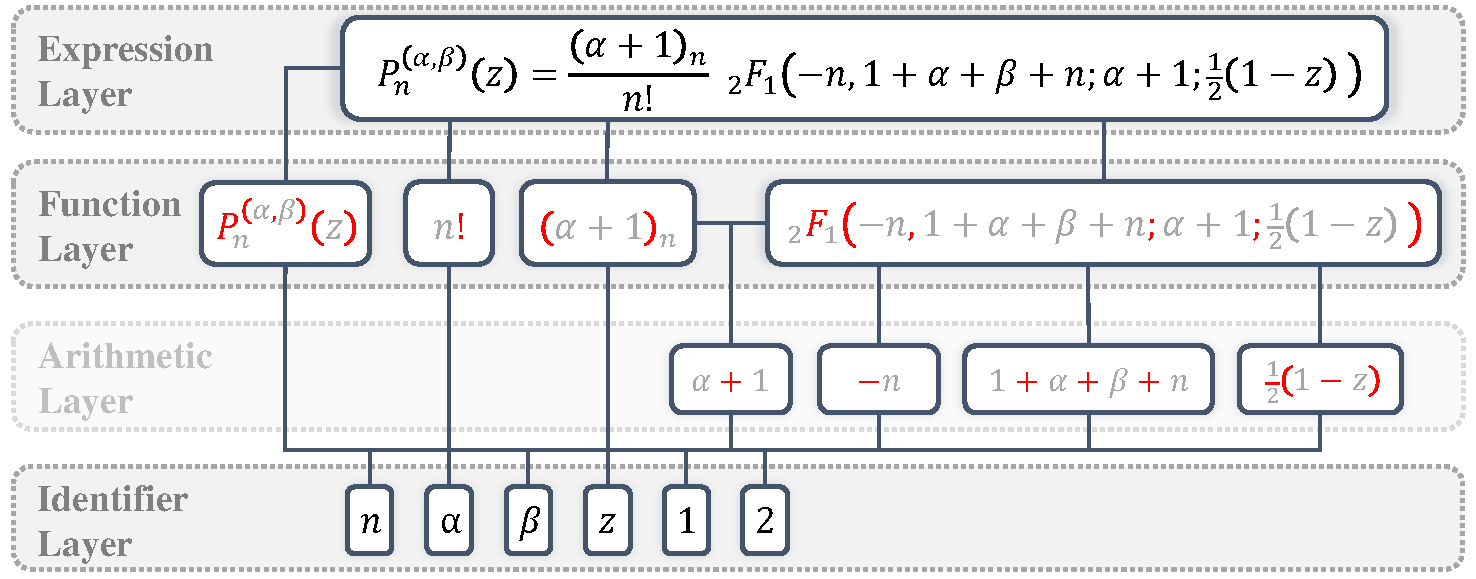
\includegraphics[width=\textwidth]{moi-layers-4L.pdf}
	\caption[Short caption for the List of Figures.]{Long caption directly below the picture.}
	\label{fig:moi-layers-4l}
\end{figure}

\pagebreak
And a lot of different information boxes. Take a look at \verb|boxexample.tex| for further details.

\begin{thesisobjectivebox}
Your thesis objective
\end{thesisobjectivebox}

\begin{researchtaskbox}{Research Tasks Box}
\begin{enumerate}[label=\textbf{\Roman*}, labelsep=1em]
\setlength\itemsep{0.25em}
\item\label{rt:I} \lipsum[1][3]
\item\label{rt:II} \lipsum[1][4]
\item\label{rt:III} \lipsum[1][5]
\item\label{rt:IV} \lipsum[1][6]
\item\label{rt:V} \lipsum[1][7]
\end{enumerate}
\end{researchtaskbox}

\begin{infobox}{Small Icon Info Box}
With additional infos.
\end{infobox}

\begin{examplebox}{Example Box}
With an example
\end{examplebox}

\begin{examplebox}{Single Line Info Box: \normalfont\mdseries With normal font following.}
\vspace*{-0.165cm}
\end{examplebox}

\paperbox{Www20-frontpage.jpg}{%
\textit{``Discovering Mathematical Objects of Interest --- A Study of Mathematical Notations''} by \textbf{Andr\'{e} Greiner-Petter}, Moritz Schubotz, Fabien M\"{u}ller, Corinna Bretinger, Howard S.~Cohl, Akiko Aizawa, and Bela Gipp. \textbf{In:} \textit{Proceedings of the Web Conference} (WWW), 2020.%
}{Chapter~\ref{ch:related-work} --- \cite{GreinerPetterSMB20}}

\begin{definitionbox}{Definition Box}[def:caption]
A nice definition box.
\end{definitionbox}

\begin{translationbox}{Translation Box}
Usually you want nice code box inside, see the next box as an example.
\end{translationbox}

\begin{translationbox}{Translation Box with Code}
\begin{code}[mytex]
P_n^{(\alpha,\beta)}(z) = \frac{(\alpha+1)_n}{n!} {}_2F_1\left(-n,1+\alpha+\beta+n;\alpha+1;\tfrac{1}{2}(1-z)\right)
\end{code}
\end{translationbox}

\begin{translationbox}{Translation Box with Custom Code}
\begin{customcode}[language=maple, mathescape=false]
diff( exp(z^2)*erfc(z), [z$(n)] ) = (-1)^(n)*(2)^(n)*factorial(n)*exp(z^2)*erfc(n, z)
\end{customcode} %$ %fool editor that the equation is "closed"
\vspace{-0.2cm}
\begin{footnotesize}
\vspace{-0.15cm}
\hfill Redundant parentheses removed to improve readability.
\end{footnotesize}
\end{translationbox}

\begin{translationbox}{Translation of Bailey’s Transformation of Very-Well-Poised ${}_{8}\phi_{7}$}
\begin{customcode}[language=mymathematica, basicstyle=\LSTfont, numbers=none, stepnumber=1, numbersep=6pt]
QHypergeometricPFQ[{a, q*(a)^(Divide[1,2]),-q*(a)^(Divide[1,2]),b,c,d,e,f},{(a)^(Divide[1,2]), -(a)^(Divide[1,2]),a*q/b,a*q/c,a*q/d,a*q/e,a*q/f},q, Divide[(a)^(2)*(q)^(2),b*c*d*e*f]] 
 == Divide[Product[QPochhammer[Part[{a*q,a*q/(d*e),a*q/(d*f),a*q/(e*f)},i],q, Infinity],{i,1, Length[{a*q,a*q/(d*e),a*q/(d*f),a*q/(e*f)}]}], Product[QPochhammer[Part[{a*q/d,a*q/e,a*q/f,a*q/(d*e*f)},i],q, Infinity],{i,1, Length[{a*q/d,a*q/e,a*q/f,a*q/(d*e*f)}]}]]* QHypergeometricPFQ[{a*q/(b*c),d,e,f},{a*q/b,a*q/c,d*e*f/a},q,q]
 + Divide[Product[QPochhammer[Part[{a*q,a*q/(b*c),d,e,f,(a)^(2)*(q)^(2)/(b*d*e*f),(a)^(2)*(q)^(2)/(c*d*e*f)},i],q, Infinity],{i,1, Length[{a*q,a*q/(b*c),d,e,f,(a)^(2)*(q)^(2)/(b*d*e*f),(a)^(2)*(q)^(2)/(c*d*e*f)}]}], Product[QPochhammer[Part[{a*q/b,a*q/c,a*q/d,a*q/e,a*q/f,(a)^(2)*(q)^(2)/(b*c*d*e*f),d*e*f/(a*q)},i],q, Infinity],{i,1, Length[{a*q/b,a*q/c,a*q/d,a*q/e, a*q/f,(a)^(2)*(q)^(2)/(b*c*d*e*f),d*e*f/(a*q)}]}]]
 * QHypergeometricPFQ[{a*q/(d*e),a*q/(d*f), a*q/(e*f),(a)^(2)*(q)^(2)/(b*c*d*e*f)},{(a)^(2)*(q)^(2)/(b*d*e*f),(a)^(2)*(q)^(2)/(c*d*e*f), a*(q)^(2)/(d*e*f)},q,q]
\end{customcode}
\vspace{-0.35cm}
\begin{footnotesize}
\hfill\rule{0.4\textwidth}{.4pt}

\vspace{-0.15cm}
\hfill Linebreaks are manually added to improve readability.
\end{footnotesize}
\end{translationbox}

\begin{codebox}{A Code Box}
\begin{code}[MathML]
<mrow>
  <msub>
    <mi>P</mi>
    <mi>n</mi>
  </msub>
  <mo>
    <!-- Invisible 
    Funct. Appl. 
    Unicode U+2061 -->  
  </mo>
  <mrow>
    <mo>(</mo>
    <mi>x</mi>
    <mo>)</mo>
  </mrow>
</mrow>
\end{code}
\end{codebox}

\begin{codebox}{A Code Box With Caption}[With Caption Text][code:caption]
\begin{code}[MathML]
<mrow></mrow>
\end{code}
\end{codebox}

\begin{codebox}{A Latex Code Box}[With caption.][lst:caption]
\begin{code}[mytex]
P_n^{(\alpha , \beta)}(x)          % Generic LaTeX
\JacobipolyP{n}{\alpha}{\beta}@{x} % Semantic LaTeX
\end{code}
\end{codebox}


\section{Example Section}\label{sec:research-gap}

\lipsum[3]

\section{Example Outline}\label{sec:outline}
\noindent\textbf{\Cref{ch:introduction}}
\lipsum[1][1-2]

\noindent\textbf{\Cref{ch:related-work}}
\lipsum[1][1-2]

\noindent\textbf{The \hyperref[ch:appendix]{Appendix}}
\lipsum[1][1-2]

\subsection{Example Overview of Publications}
\lipsum[2]

\begin{table}[ht]
\caption[Example of short caption for the List of Tables.]{Example full caption of a table.}
\label{tab:publications}
\centering
\renewcommand{\arraystretch}{1.1}
\begin{tabular}{c:l:l:l:l:c:l:r}\hline
	\textbf{Ch.} & \textbf{Venue} & \textbf{Year} & \textbf{Type} & \textbf{Length} & \makecell[bl]{\textbf{Author} \\\textbf{Position}} & \makecell[bl]{\textbf{Venue} \\\textbf{Rating}} & \textbf{Ref.} \\\hline
	\rowcolor{TableRowColor}\multirow{2}{*}{\cellcolor{white}\ref{ch:related-work}} 
	& \gls{scientometrics} & 2020 & Journal & Full & 1 of 7 & SJR Q1 & \cite{GreinerPetterYRM20} \\
	& \gls{www} & 2020 & Conference & Full & 1 of 7 & \glslink{core}{Core} A* & \cite{GreinerPetterSMB20} \\
 	\hline
\end{tabular}
\end{table}


% If you want to add a manual pagebreak between the chapters in the table of contents, use the following
% command:
%\addtocontents{toc}{\protect\pagebreak}

\chapter{Related Work}\label{ch:related-work}
\minitoc% creates toc for this chapter
\chapterQuote{%
I don't know half of you half as well as I should like, and I like less than half of you half as well as you deserve.
}{Bilbo Baggins - \textit{The Lord of the Rings}}

\lipsum[6]

\section{Background and Overview}\label{sec:formats-intro}

\section{Formats and Conversions}\label{sec:fomats}

\section{Presentation and Content}\label{sec:pres-and-content}

\subsection{Subsection}

\subsubsection{Subsubsection}

\paragraph{Paragraph}

\subsubsection{Subsubsection}

\subsection{Subsection 2}

\subsection{Subsection 3}

\section{Closing Section}\label{sec:closing}


% Start of backmatter
\pagebreak
\makeatletter
\let\@chapterQuote\@empty
\makeatother

\backmatter
\appendix
\titlespacing*{\chapter}{0pt}{-20pt}{40pt}
\renewcommand\chaptername{Appendix}
\renewcommand\thesection{\Alph{section}}
\renewcommand\currentmattertitle{}

%\setcounter{secnumdepth}{-1}
\cleardoublepage
\phantomsection
\addcontentsline{toc}{chapter}{BACK MATTER }
%\pagestyle{plain}
%\chapter*{BACK MATTER}
%\adjustmtc
%\minitoc

%\cleardoublepage
\phantomsection
\addcontentsline{toc}{section}{Appendix}
\addtocontents{lof}{\protect\addvspace{10pt}} %adds 10pt space in list of figures
\renewcommand\currentmattertitle{Back Matter}
\chapter*{Appendix}\label{ch:appendix}
\adjustmtc
\minitoc
%since we use chapter*, classical counters getting confused.
% we want equations, figures, tables, and lstlistings to reflect 
% the appendix in the label. So we need to update all counter labels and reset them to 0
%\renewcommand\thesection{\Alph{section}}
\renewcommand\thefigure{\thesection.\arabic{figure}}
\renewcommand\thelstlisting{\thesection.\arabic{lstlisting}}
\renewcommand\thetable{\thesection.\arabic{table}}
\renewcommand\theequation{\thesection.\arabic{equation}}
\setcounter{figure}{0}
\setcounter{lstlisting}{0}
\setcounter{table}{0}
\setcounter{equation}{0}
\markboth{{\bfseries Appendix}}{}

\lipsum[3]

\section{My First Appendix}\label{sec:app:test1}

\section{Another Appendix}\label{sec:app:test2}

\section{Appendix With Subsections}\label{sec:app:test3}

\subsection{A Nested Subsection}

\subsubsection{With Subsubsections}

\paragraph{And a Paragraph}

\subsection{Another Subsection}

\subsection{And Another}

\section{My Last Appendix}\label{sec:app:test4}


%\phantomsection
%\addcontentsline{toc}{section}{Abbreviation}
%\printglossary[type=\acronymtype]

\cleardoublepage
\phantomsection
\addcontentsline{toc}{section}{Glossary}
\pagestyle{othermatter}
\setglossarystyle{thesislist}
\printglossary

\cleardoublepage
\phantomsection
\addcontentsline{toc}{section}{Bibliography of Publications, Submissions \& Talks}\label{backmatter:pubs}
\renewcommand*{\bibfont}{\footnotesize} % make it very small
\defbibnote{mybib}{\markboth{\bfseries Bibliography of Publications, Submissions \& Talks}{}}

\Setmaxbibnames{99}
\printbibliography[keyword=primary, title={Bibliography of Publications,\\ Submissions \& Talks}, prenote=mybib]

\cleardoublepage
\phantomsection
\addcontentsline{toc}{section}{Bibliography}
\renewcommand*{\bibfont}{\footnotesize} % make it very small
\defbibnote{dissbib}{\markboth{\bfseries Bibliography}{}}
\Setmaxbibnames{6}
\printbibliography[notkeyword=primary, prenote=dissbib]

\end{document}